\documentclass[12pt]{article}

\usepackage{amsmath,amssymb,amsfonts,mathtools}
\usepackage{physics}
\usepackage{bm}
\usepackage{geometry}
\usepackage{graphicx}
\usepackage{hyperref}
\usepackage{mathrsfs}
\usepackage{tensor}
\usepackage{cite}
\usepackage{setspace}
\usepackage{titlesec}
\usepackage{tikz}
\usepackage{pgfplots}
% pgfplotsset loaded below
\pgfplotsset{compat=1.18}
\usetikzlibrary{arrows.meta,decorations.pathmorphing,decorations.markings,
                calc,shapes.geometric,fit,backgrounds,positioning,
                decorations.pathreplacing,patterns}
\usepackage{xcolor}
\usepackage{booktabs}
\usepackage{array}
\usepackage{caption}
\usepackage{subcaption}
\usepackage{enumitem}
\usepackage{cleveref}
\usepackage{thmtools}
\usepackage{amsthm}
\usepackage{mdframed}

\geometry{margin=1in, top=1.1in, bottom=1.1in}
\setstretch{1.18}

%% Theorem environments
\newtheorem{theorem}{Theorem}[section]
\newtheorem{proposition}[theorem]{Proposition}
\newtheorem{corollary}[theorem]{Corollary}
\newtheorem{lemma}[theorem]{Lemma}
\theoremstyle{definition}
\newtheorem{definition}[theorem]{Definition}
\newtheorem{remark}[theorem]{Remark}

%% Custom colors
\definecolor{rsvpblue}{RGB}{30,80,160}
\definecolor{axiongray}{RGB}{90,90,90}
\definecolor{coherentgreen}{RGB}{20,130,80}
\definecolor{washoutred}{RGB}{180,40,40}

\hypersetup{
  colorlinks=true,
  linkcolor=rsvpblue,
  citecolor=coherentgreen,
  urlcolor=rsvpblue
}

%% Shorthand macros
\newcommand{\kA}{\kappa_A}
\newcommand{\Wrec}{\Delta\eta_{\mathrm{rec}}}
\newcommand{\xirec}{\xi_{\mathrm{rec}}}
\newcommand{\betaobs}{\beta_{\mathrm{obs}}}
\newcommand{\etaLSS}{\eta_{\mathrm{LSS}}}
\newcommand{\etastar}{\eta_\star}
\newcommand{\etaobs}{\eta_0}
\newcommand{\Wpm}{\mathcal{W}_\pm}
\newcommand{\VarW}{\mathrm{Var}_W}
\newcommand{\EW}{\mathbb{E}_W}
\newcommand{\PLSSphi}{\phi_\star}
\newcommand{\gpg}{g_{\phi\gamma}}
\newcommand{\RSVP}{\textsc{rsvp}}
\newcommand{\plenum}{\widetilde{\Gamma}}

%% Section title formatting
\titleformat{\section}{\large\bfseries\color{rsvpblue}}{{\thesection}}{1em}{}
\titleformat{\subsection}{\normalsize\bfseries}{{\thesubsection}}{1em}{}

%%-------------------------------------------------------------------
\title{\textbf{Axial Holonomy and Visibility-Weighted Coherence:\\[4pt]
Cosmic Birefringence in the Relativistic Scalar--Vector Plenum}}

\author{Flyxion}

\date{\today}

\begin{document}
\maketitle
\thispagestyle{empty}

\begin{abstract}
Cosmic birefringence, the rotation of CMB polarization by an angle
$\beta\sim 0.3^\circ$ detected at high significance in recent data
\cite{MinamiKomatsu2020,Eskilt2022,Diego-Palazuelos2023},
is typically attributed to a Chern--Simons coupling between photons
and axion-like particles (ALPs) \cite{Carroll1990,Lue1999}.
Here we reinterpret this phenomenon within the
Relativistic Scalar--Vector Plenum (RSVP)
as a \emph{visibility-weighted axial holonomy} of a
parity-odd sector of the plenum connection.
The polarization rotation angle is the integral of an effective axial
connection $\kappa_A$ along null geodesics;
the washout suppression of polarization amplitude arises from
phase-variance of $\kappa_A$ across the finite recombination visibility
kernel $W(\eta)$ \cite{Fujita2021,Sherfield2023}.
We derive a transport formalism in which mean rotation and depolarization
are governed respectively by the first and second spectral moments of the
axial connection.
The two-field ALP mechanism of Shao--Obata--Zhang \cite{ShaoObataZhang2025}
emerges as a special case of a multi-modal axial sector whose independent
phase components factorize under visibility averaging, yielding the
familiar $\sqrt{N}$ relaxation of washout constraints through variance additivity.
A continuous synchronization model for the parity-odd phase field leads to
a \emph{coherence theorem}: the CMB polarization amplitude imposes a lower
bound on the axial correlation length at $z\approx1100$.
This reframing replaces particle-specific exclusion statements with a
geometric coherence inequality, reveals structural equivalence between
cosmological birefringence and phase-stable photonic computation
\cite{Ozawa2019,Joannopoulos2008}, and predicts discriminants absent
in minimal axion models, including correlations between birefringence
anisotropies and entropy gradients, vorticity statistics, and
multipole-dependent depolarization.
Cosmic birefringence is thus recast as a probe of axial synchronization
in the universe's parity-odd sector rather than solely as evidence for
a propagating pseudoscalar field.
\end{abstract}

\vspace{2pt}
\noindent\rule{\textwidth}{0.4pt}
\tableofcontents
\vspace{4pt}
\noindent\rule{\textwidth}{0.4pt}

\newpage

%%====================================================================
\section{Introduction}
\label{sec:intro}
%%====================================================================

Recent high-significance measurements of cosmic microwave background (CMB)
polarization have revived interest in the possibility of a nonzero global
birefringence angle.
The Planck, WMAP, and ACT data-sets together indicate a rotation
$\beta \approx 0.35^\circ$ at roughly $3\sigma$ significance
\cite{MinamiKomatsu2020,Eskilt2022,Diego-Palazuelos2023,ACTPol2024},
with anisotropic components beginning to be resolved at degree angular scales.
Conventionally, such rotation is modeled through a Chern--Simons coupling
\begin{equation}
  \mathcal{L}_{\mathrm{CS}}
  = -\frac{\gpg}{4}\,\phi\,F_{\mu\nu}\widetilde{F}^{\mu\nu},
  \label{eq:CS_action}
\end{equation}
which leads to a polarization angle proportional to the ALP field
displacement between emission and observation \cite{Carroll1990,Lue1999,
Finelli2009,Pospelov2009}.
Within that framework, the observational bound on polarization amplitude
constrains the oscillation rate and coupling of the pseudoscalar through a
washout condition arising from the finite thickness of recombination
\cite{Fujita2021,Sherfield2023,Murai2023}.

While this particle-based interpretation is algebraically sufficient, it is
not logically necessary.
The observable quantity is a rotation of the photon's transverse polarization
frame, accumulated along null geodesics and weighted by the visibility
function of recombination \cite{Zaldarriaga1998,Hu1997}.
At a structural level this is a \emph{holonomy problem}:
polarization is parallel-transported by an effective optical connection,
and birefringence measures the parity-odd component of that connection
integrated along the path.
The washout bound constrains not a field species per se
but the \emph{phase coherence} of whatever geometric sector sources that
parity-odd projection across the emission kernel.

In this paper we develop that geometric interpretation within the
Relativistic Scalar--Vector Plenum (RSVP) framework.
RSVP posits that cosmological dynamics are governed not solely by a metric
tensor but by a coupled scalar--vector--entropy system $(\Phi,v^\mu,S)$
defined on spacetime \cite{Penrose2004,Verlinde2011,Jacobson1995}.
Gravitational and optical phenomena emerge from the combined geometry of
these fields through effective connections constructed from their gradients
and contractions.
Parity-odd structures arise naturally from pseudoscalar combinations such as
$\varepsilon_{\mu\nu\rho\sigma} k^\mu u^\nu \nabla^\rho S\, v^\sigma$,
where $k^\mu$ is the photon wavevector and $u^\mu$ a comoving four-velocity
\cite{Alexander2009,Nair2010}.

\paragraph{Main results.}
\begin{enumerate}[leftmargin=1.8em,itemsep=2pt]
  \item We derive an \emph{axial transport law} (\cref{sec:geometry})
        expressing CMB polarization rotation as the holonomy of a
        parity-odd sector of the RSVP plenum connection.
  \item We establish a \emph{visibility-weighted holonomy formalism}
        (\cref{sec:visibility}) that identifies the washout bound with a
        spectral coherence constraint on $\kA$.
  \item We show that the two-field ALP mechanism of
        \cite{ShaoObataZhang2025} is a \emph{special case}
        (\cref{sec:multimodal}) of multi-modal axial coherence
        governed by variance additivity.
  \item We prove a \emph{coherence theorem} (\cref{sec:synchronization,
        sec:continuous}) bounding the axial correlation length at
        recombination.
  \item We derive an \emph{entropy--coherence inequality}
        (\cref{sec:entropy}) unifying cosmological washout with the
        thermodynamic cost of phase-stable computation.
  \item We identify \emph{observational discriminants}
        (\cref{sec:discriminants}) that distinguish geometric axial
        coherence from free pseudoscalar transport.
\end{enumerate}

\medskip
The paper is organized as follows.
\Cref{sec:geometry} develops the RSVP optical connection and axial
holonomy.
\Cref{sec:visibility} establishes the visibility-weighted formalism and
coherence constraints.
\Cref{sec:multimodal} treats multi-modal factorization and the two-field
mechanism.
\Cref{sec:boundary} discusses foliation structure and local-field dominance.
\Cref{sec:synchronization} introduces the 5D Ising synchronization model.
\Cref{sec:continuous} derives the continuous axial phase model and states
the coherence theorem.
\Cref{sec:entropy} establishes the entropy--coherence inequality and its
implications for photonic computing.
\Cref{sec:discriminants} presents observational discriminants.
\Cref{sec:conclusion} synthesizes the results.
Technical derivations occupy Appendices \ref{app:transport}--\ref{app:MSR}.

%%====================================================================
\section{Geometric Structure of the Relativistic Scalar--Vector Plenum}
\label{sec:geometry}
%%====================================================================

\subsection{Plenum fields and the RSVP connection}

The Relativistic Scalar--Vector Plenum (RSVP) is a geometric field theory
in which spacetime carries three interlocking fields: a scalar density
$\Phi$, a vector flow $v^\mu$, and an entropy density $S$.
The metric $g_{\mu\nu}$ is interpreted as an emergent large-scale descriptor
of averaged plenum structure rather than a primitive background variable
\cite{Jacobson1995,Verlinde2011,Padmanabhan2010}.
Deviations from Levi--Civita transport arise from gradients and vorticity of
$(\Phi,v^\mu,S)$.

The full plenum connection is
\begin{equation}
  \plenum^\mu{}_{\nu\rho}
  = \Gamma^\mu{}_{\nu\rho}
  + \Delta^\mu{}_{\nu\rho}(\Phi,v,S),
  \label{eq:plenum_connection}
\end{equation}
where $\Delta^\mu{}_{\nu\rho}$ represents non-Riemannian structure induced
by plenum ordering \cite{Cartan1922,Hehl1976}.
The correction decomposes irreducibly under spatial inversion into
parity-even and parity-odd sectors.
The parity-odd sector, which we denote $\Delta^{(\mathrm{odd})}$, acts
differently on left- and right-handed polarization states; it is the
geometric locus of cosmic birefringence in RSVP.

\begin{figure}[h]
\centering
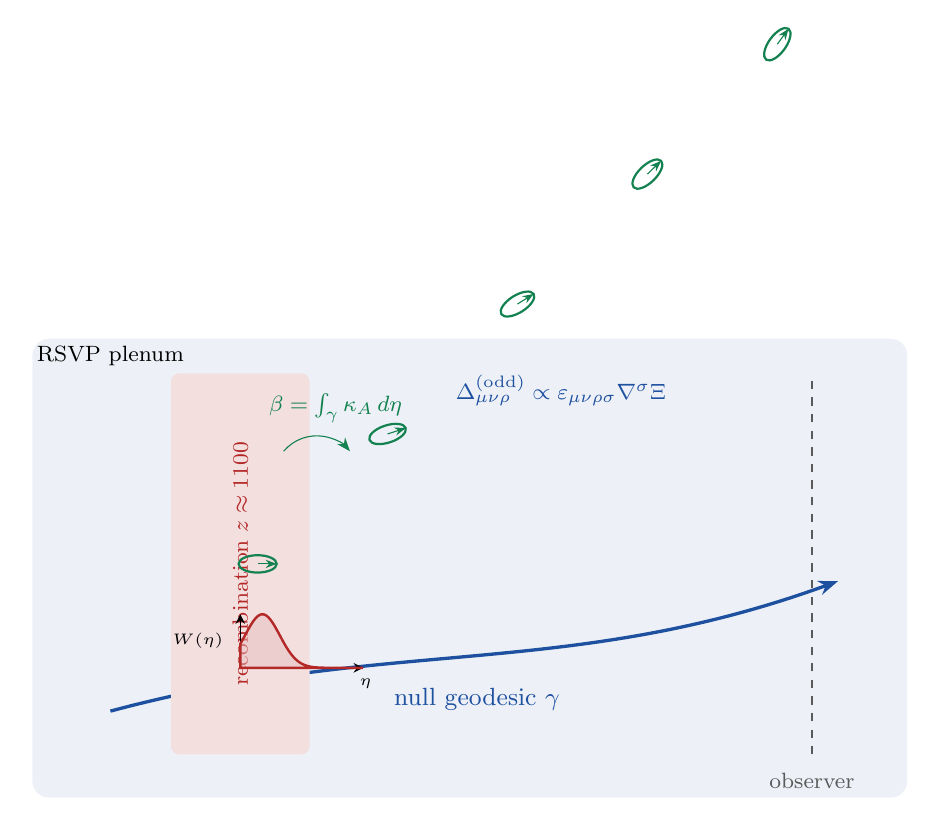
\begin{tikzpicture}[scale=1.1,
  every node/.style={font=\small},
  arrow/.style={-{Stealth[length=6pt]},thick}]

  %% Spacetime background stripe
  \fill[rsvpblue!8, rounded corners=6pt]
    (-0.6,-0.5) rectangle (9.5,4.8);

  %% Null geodesic
  \draw[rsvpblue, very thick, -{Stealth[length=7pt]}]
    (0.3,0.5) to[out=15,in=200] node[midway,below=8pt,rsvpblue]
    {null geodesic $\gamma$} (8.7,2.0);

  %% LSS band
  \fill[washoutred!15, rounded corners=3pt]
    (1.0,0.0) rectangle (2.6,4.4);
  \node[washoutred, rotate=90, font=\footnotesize] at (1.8,2.2)
    {recombination $z\approx1100$};

  %% Observer vertical line
  \draw[axiongray, dashed, thick] (8.4,0.0) -- (8.4,4.4);
  \node[axiongray, font=\footnotesize] at (8.4,-0.3) {observer};

  %% Polarization ellipses along ray
  \foreach \x/\ang in {2.0/0, 3.5/18, 5.0/32, 6.5/44, 8.0/54}{
    \begin{scope}[shift={(\x, 0.5+(\x-0.3)*0.178)}, rotate=\ang]
      \draw[coherentgreen, thick] (0,0) ellipse (0.22 and 0.10);
      \draw[coherentgreen,-{Stealth[length=4pt]},thin]
        (0,0) -- (0.22,0);
    \end{scope}
  }

  %% Rotation annotation
  \draw[coherentgreen, -{Stealth[length=5pt]}]
    (2.3,3.5) arc(140:40:0.5);
  \node[coherentgreen, font=\footnotesize] at (2.9,4.0)
    {$\beta = \int_\gamma \kA\,d\eta$};

  %% Visibility kernel inset
  \begin{axis}[
    at={(1.8cm,1.0cm)}, anchor=south west,
    width=3.0cm, height=2.2cm,
    axis x line=bottom, axis y line=left,
    xtick=\empty, ytick=\empty,
    xlabel={\tiny $\eta$},
    ylabel={\tiny $W(\eta)$},
    xlabel style={font=\tiny, at={(axis description cs:1.02,0.0)}},
    ylabel style={font=\tiny, rotate=-90},
    domain=0:1, samples=80,
    clip=false
  ]
    \addplot[washoutred, thick, fill=washoutred!30, fill opacity=0.5]
      {exp(-25*(x-0.18)^2)} \closedcycle;
  \end{axis}

  %% Labels
  \node[font=\footnotesize] at (0.3,4.6) {RSVP plenum};
  \node[font=\footnotesize,rsvpblue] at (5.5,4.2)
    {$\Delta^{(\mathrm{odd})}_{\mu\nu\rho}\propto
      \varepsilon_{\mu\nu\rho\sigma}\nabla^\sigma\Xi$};
\end{tikzpicture}
\caption{Schematic of axial holonomy along a null geodesic $\gamma$
  in the RSVP plenum.
  Photon polarization (green ellipses) rotates by an angle
  $\beta=\int_\gamma\kA\,d\eta$ controlled by the parity-odd projection
  $\kA$ of the plenum connection $\Delta^{(\mathrm{odd})}$.
  The red band marks the recombination visibility kernel $W(\eta)$;
  phase oscillations faster than $\Wrec$ contribute to depolarization
  rather than coherent rotation.}
\label{fig:holonomy_schematic}
\end{figure}

\subsection{Polarization transport equation}

Let $k^\mu$ be the null tangent to $\gamma$ and $P^\mu$ a transverse
polarization vector with $P^\mu k_\mu=0$.
Standard geometric optics gives $k^\nu\nabla_\nu P^\mu=0$
\cite{MisnerThorneWheeler,Grasso2018,Oancea2020};
in RSVP the transport is instead
\begin{equation}
  k^\nu\widetilde{\nabla}_\nu P^\mu = 0,
\end{equation}
where $\widetilde{\nabla}$ uses the full plenum connection
\eqref{eq:plenum_connection}.
Projecting onto the two-dimensional screen bundle
$\{e_1^\mu,e_2^\mu\}$ orthogonal to $k^\mu$ and $u^\mu$, the parity-odd
sector induces an effective scalar angular velocity
\begin{equation}
  \frac{d\theta}{d\lambda} = \kA(\lambda),
  \qquad
  \kA(\lambda)
  = \Pi^\mu{}_a\,\Pi^\nu{}_b\,\epsilon^{ab}\,k^\rho
    \Delta_{\mu\nu\rho}^{(\mathrm{odd})},
  \label{eq:kA_def}
\end{equation}
so that the accumulated axial holonomy along $\gamma$ is
\begin{equation}
  \boxed{
  H_A[\gamma]
  = \int_{\etaLSS}^{\etaobs}
    \kA(\eta,x(\eta))\,d\eta.}
  \label{eq:holonomy}
\end{equation}
This is structurally identical to the Chern--Simons result
$\beta=\frac{1}{2}\gpg(\phi_{\etaobs}-\phi_{\etaLSS})$
under the identification
\begin{equation}
  \kA \;\longleftrightarrow\; \tfrac{1}{2}\gpg\,\partial_\eta\phi,
  \label{eq:identification}
\end{equation}
but now $\kA$ is a projection of plenum geometry rather than a derivative
of a particle field.

\subsection{Internal origin of the parity-odd sector}

A minimal covariant parity-odd connection compatible with RSVP fields is
\begin{equation}
  \Delta^{(\mathrm{odd})}_{\mu\nu\rho}
  = \alpha\,\varepsilon_{\mu\nu\rho\sigma}\,\nabla^\sigma\Xi(\Phi,v,S),
  \label{eq:Delta_odd}
\end{equation}
where $\alpha$ is a coupling scale and $\Xi$ is any pseudoscalar functional
of the plenum.
The canonical choice coupling entropy gradients to vorticity is
\begin{equation}
  \Xi = \nabla_\mu S\,\omega^\mu,
  \qquad
  \omega^\mu = \varepsilon^{\mu\nu\rho\sigma}u_\nu\nabla_\rho v_\sigma,
  \label{eq:Xi}
\end{equation}
which is manifestly parity-odd and depends only on plenum kinematics,
not on any new fundamental field
\cite{Alexander2009,Nair2010,Maleknejad2013}.
The axion model is recovered when $\Xi\to\phi$ is promoted to an independent
dynamical pseudoscalar with the action \eqref{eq:CS_action}.
RSVP treats $\Xi$ as emergent from plenum ordering.

%%====================================================================
\section{Visibility-Weighted Holonomy and Coherence Constraints}
\label{sec:visibility}
%%====================================================================

\subsection{Observable polarization}

CMB polarization is generated across a finite conformal time interval
centered at recombination \cite{Zaldarriaga1998,Hu1997,Kosowsky1996}.
Let $W(\eta)$ be the visibility function, normalized to unity, with
characteristic width $\Wrec\approx10\,\mathrm{Mpc}/h$ at
$z\approx1100$ \cite{Weinberg2008}.
Defining complex polarization $P_\pm=Q\pm iU$, the observed polarization is
\begin{equation}
  P_\pm^{\mathrm{obs}}(\hat{n})
  = \int d\eta\,W(\eta)\,
    e^{\pm 2i\beta(\eta,\hat{n})}\,P_\pm^{(0)}(\eta,\hat{n}),
  \label{eq:Pobs}
\end{equation}
where $\beta(\eta,\hat{n})=\int_\eta^{\etaobs}\kA(\eta',x(\eta'))d\eta'$
is the holonomy from emission time $\eta$ to the observer.
Factoring out the slowly varying intrinsic polarization,
\begin{equation}
  P_\pm^{\mathrm{obs}} = \Wpm(\hat{n})\,P_\pm^{(0)}(\etastar,\hat{n}),
  \quad
  \Wpm(\hat{n}) = \int d\eta\,W(\eta)\,e^{\pm2i\beta(\eta,\hat{n})}.
  \label{eq:Wpm}
\end{equation}
The washout effect is $|\Wpm|<1$ due to phase decoherence across
the kernel \cite{Fujita2021,Sherfield2023,Murai2023}.

\subsection{Spectral decomposition and Bessel suppression}

Decompose $\kA$ into a coherent component and oscillatory modes:
\begin{equation}
  \kA(\eta) = \kappa_0(\eta)
    + \sum_k a_k\cos(\omega_k\eta+\varphi_k).
  \label{eq:kA_decomp}
\end{equation}
The holonomy becomes
\begin{equation}
  \beta(\eta) = \bar\beta
    + \sum_k A_k\sin(\omega_k\eta+\varphi_k),
  \qquad
  A_k=\frac{a_k}{\omega_k},
  \label{eq:beta_decomp}
\end{equation}
where $\bar\beta=\int_{\etastar}^{\etaobs}\kappa_0d\eta'$.
For modes with $\omega_k\Wrec\gg1$ the integral over $W(\eta)$
reduces to a Bessel-$J_0$ suppression
\cite{Abramowitz1972,Watson1944}:
\begin{equation}
  \int d\eta\,W(\eta)\,e^{iA_k\sin(\omega_k\eta)}
  \approx J_0(A_k).
\end{equation}
With spectrally separated modes, the full suppression factorizes:
\begin{equation}
  \Wpm \approx e^{\pm2i\bar\beta}\prod_k J_0(2A_k).
  \label{eq:Wpm_bessel}
\end{equation}
Expanding for small $A_k$:
\begin{equation}
  |\Wpm| \approx 1 - 2\sum_k A_k^2 + \mathcal{O}(A_k^4),
  \label{eq:Wpm_expand}
\end{equation}
yielding the fundamental \emph{coherence inequality}
\begin{equation}
  \boxed{
  \sum_k A_k^2 \lesssim \epsilon_{\mathrm{wash}},}
  \label{eq:coherence_ineq}
\end{equation}
where $\epsilon_{\mathrm{wash}}$ is the observationally determined upper bound
on depolarization \cite{MinamiKomatsu2020,Eskilt2022,Sherfield2023}.
This bounds the spectral variance of $\kA$ at
frequencies exceeding $\Wrec^{-1}$, not the mean coherent component
$\bar\beta$.

\begin{figure}[h]
\centering
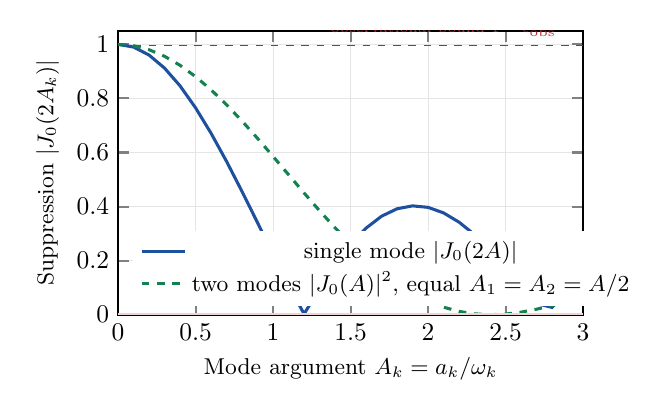
\begin{tikzpicture}[scale=0.92]
  \begin{axis}[
    width=8cm, height=5.5cm,
    xlabel={Mode argument $A_k = a_k/\omega_k$},
    ylabel={Suppression $|J_0(2A_k)|$},
    xmin=0, xmax=3.0,
    ymin=0, ymax=1.05,
    xtick={0,0.5,1.0,1.5,2.0,2.5,3.0},
    ytick={0,0.2,0.4,0.6,0.8,1.0},
    grid=both,
    grid style={draw=gray!20},
    legend pos=south west,
    legend style={font=\small, draw=none, fill=white},
    axis line style={thick},
    tick style={thick},
    label style={font=\small},
  ]
    %% Single-field J0 (precomputed from scipy)
    \addplot[rsvpblue, very thick]
      coordinates {
        (0.0,1.0)(0.1,0.99)(0.2,0.9604)(0.3,0.912)(0.4,0.8463)
        (0.5,0.7652)(0.6,0.6711)(0.7,0.5669)(0.8,0.4554)(0.9,0.34)
        (1.0,0.2239)(1.1,0.1104)(1.2,0.0025)(1.3,0.0968)(1.4,0.185)
        (1.5,0.2601)(1.6,0.3202)(1.7,0.3643)(1.8,0.3918)(1.9,0.4026)
        (2.0,0.3971)(2.1,0.3766)(2.2,0.3423)(2.3,0.2961)(2.4,0.2404)
        (2.5,0.1776)(2.6,0.1103)(2.7,0.0412)(2.8,0.027)(2.9,0.0917)
        (3.0,0.1506)};
    \addlegendentry{single mode $|J_0(2A)|$}

    %% Two-field product (equal amplitudes, precomputed)
    \addplot[coherentgreen, very thick, dashed]
      coordinates {
        (0.0,1.0)(0.1,0.995)(0.2,0.9801)(0.3,0.9558)(0.4,0.9224)
        (0.5,0.8807)(0.6,0.8318)(0.7,0.7765)(0.8,0.7162)(0.9,0.6521)
        (1.0,0.5855)(1.1,0.5179)(1.2,0.4504)(1.3,0.3845)(1.4,0.3213)
        (1.5,0.262)(1.6,0.2074)(1.7,0.1584)(1.8,0.1156)(1.9,0.0794)
        (2.0,0.0501)(2.1,0.0278)(2.2,0.0122)(2.3,0.0031)(2.4,0.0)
        (2.5,0.0023)(2.6,0.0094)(2.7,0.0203)(2.8,0.0342)(2.9,0.0503)
        (3.0,0.0676)};
    \addlegendentry{two modes $|J_0(A)|^2$, equal $A_1=A_2=A/2$}

    %% Observational bound region
    \addplot[fill=washoutred!20, draw=none, domain=0:3, samples=2]
      {0.0058} \closedcycle;
    \draw[washoutred, dashed] (axis cs:0,0.9942) -- (axis cs:3,0.9942)
      node[pos=0.7, above, font=\tiny, washoutred]
      {observational bound $1-\epsilon_\mathrm{obs}$};
  \end{axis}
\end{tikzpicture}
\caption{Washout suppression factor as a function of mode amplitude $A_k$.
  Blue: single-mode Bessel factor $|J_0(2A)|$.
  Green dashed: two-mode product $|J_0(A)|^2$ for equal-amplitude modes
  each contributing $A_k=A/2$.
  The two-mode configuration achieves the same mean rotation at reduced
  depolarization.
  The red dashed line marks the observational amplitude bound
  $|\mathcal{W}_\pm|\geq0.9942$ from \protect\cite{Sherfield2023}.}
\label{fig:bessel_washout}
\end{figure}

%%====================================================================
\section{Multi-Modal Axial Connection and Factorized Dephasing}
\label{sec:multimodal}
%%====================================================================

\subsection{Two-field mechanism as special case}

In the Shao--Obata--Zhang scenario \cite{ShaoObataZhang2025}, two ALP
fields $\phi_1,\phi_2$ with common photon coupling contribute
\begin{equation}
  \kA(\eta) = -\tfrac{1}{2}\gpg
    \sum_{i=1}^2\Phi_i m_i\sin(m_i\eta+\alpha_i),
  \label{eq:kA_twofield}
\end{equation}
with mode amplitudes $A_i=\tfrac{1}{2}\gpg\Phi_i$ and
frequencies $\omega_i=m_i$.
When $|m_1-m_2|\gg\Wrec^{-1}$, cross-terms average out and
\begin{equation}
  \Wpm \approx e^{\pm2i\bar\beta}\,J_0(2A_1)\,J_0(2A_2).
  \label{eq:Wpm_twofield}
\end{equation}
This is the RSVP multi-modal result \eqref{eq:Wpm_bessel} for $k=1,2$:
the two-field mechanism is a special instance of a two-mode axial sector.

\subsection{Variance additivity and the $\sqrt{N}$ relief}

For small amplitudes, the distinction between single- and two-mode washout
is algebraic:
\begin{align}
  \text{single mode:}&
    \quad J_0(2A)\approx1-2A^2,
    \quad A=A_1+A_2,
    \label{eq:single_small}\\
  \text{two modes:}&
    \quad J_0(2A_1)J_0(2A_2)\approx1-2(A_1^2+A_2^2).
    \label{eq:two_small}
\end{align}
The single-mode suppression at fixed total amplitude scales as
$(A_1+A_2)^2$; the two-mode product scales as $A_1^2+A_2^2$.
The difference $2A_1A_2$ is the cross-term that vanishes when the modes
oscillate incoherently across the visibility kernel.
For equal amplitudes $A_1=A_2\equiv\bar{A}$,
\begin{equation}
  \frac{\text{two-mode washout}}{\text{single-mode washout}}
  = \frac{2\bar{A}^2}{4\bar{A}^2} = \tfrac{1}{2},
\end{equation}
giving a $\sqrt{2}$ improvement in coherent rotation per unit depolarization
budget.
For $N$ equal-amplitude modes:
\begin{equation}
  \frac{\langle\beta\rangle}{\sqrt{\VarW[\Theta]}}
  \propto \sqrt{N}.
  \label{eq:sqrtN}
\end{equation}
This is not a special property of axions but a \emph{universal consequence
of variance additivity under independent phase modes} \cite{Rice1954,Papoulis1991}.

\begin{figure}[h]
\centering
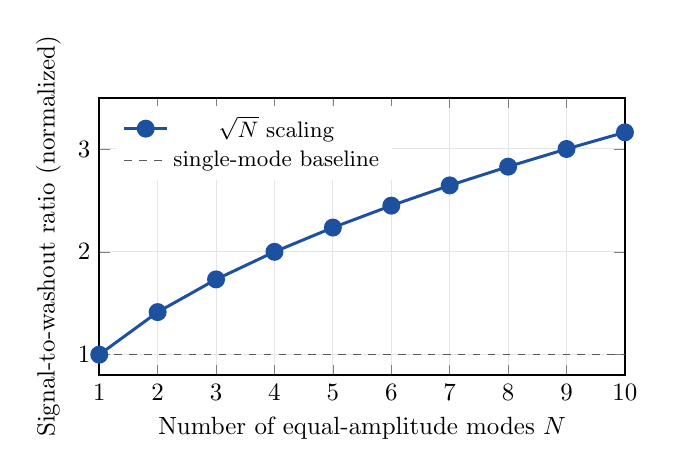
\begin{tikzpicture}[scale=0.90]
  \begin{axis}[
    width=9cm, height=5.5cm,
    xlabel={Number of equal-amplitude modes $N$},
    ylabel={Signal-to-washout ratio (normalized)},
    xmin=1, xmax=10,
    ymin=0.8, ymax=3.5,
    xtick={1,2,3,4,5,6,7,8,9,10},
    grid=both,
    grid style={draw=gray!20},
    legend pos=north west,
    legend style={font=\small, draw=none},
    axis line style={thick},
  ]
    \addplot[rsvpblue, very thick, mark=*, mark size=3pt,
             mark options={fill=rsvpblue}]
      coordinates {
        (1,1.0)(2,1.414)(3,1.732)(4,2.0)(5,2.236)
        (6,2.449)(7,2.646)(8,2.828)(9,3.0)(10,3.162)
      };
    \addlegendentry{$\sqrt{N}$ scaling}
    \addplot[axiongray, dashed, domain=1:10, samples=10]
      {1.0};
    \addlegendentry{single-mode baseline}
  \end{axis}
\end{tikzpicture}
\caption{Signal-to-washout ratio $\langle\beta\rangle/\sqrt{\VarW[\Theta]}$
  normalized to unity for $N=1$, showing universal $\sqrt{N}$ scaling
  from variance additivity under $N$ independent axial modes.
  The two-field mechanism of \protect\cite{ShaoObataZhang2025}
  corresponds to $N=2$.}
\label{fig:sqrtN}
\end{figure}

%%====================================================================
\section{Boundary Dominance and Foliation Structure}
\label{sec:boundary}
%%====================================================================

\subsection{Origin of the boundary-term structure}

The standard axion result $\beta=\tfrac{1}{2}\gpg(\phi_{\etaobs}-\phi_{\etaLSS})$
is a boundary term.
Within RSVP this structure is not an artifact of the axion equation of motion
but a \emph{structural consequence of visibility-weighted holonomy}.

Interchanging integration order in $\betaobs=\int W(\eta)\beta(\eta)d\eta$:
\begin{equation}
  \betaobs
  = \int\kA(\eta')\,\mathcal{F}(\eta')\,d\eta',
  \qquad
  \mathcal{F}(\eta') = \int_{\etaLSS}^{\eta'} W(\eta)\,d\eta.
  \label{eq:boundary_deriv}
\end{equation}
The cumulative visibility $\mathcal{F}(\eta')$ rises sharply from
$0$ to $1$ across $\Wrec$ and remains unity thereafter.
For oscillatory modes with $\omega_k\Wrec\gg1$, the emission-window
contribution $\int_{\etaLSS}^{\etastar}\kA\,\mathcal{F}\,d\eta'$ averages to
zero, leaving
\begin{equation}
  \betaobs \approx \int_{\etastar}^{\etaobs}\kA(\eta')\,d\eta',
  \label{eq:boundary_result}
\end{equation}
a \emph{post-recombination} integral depending on the observer-side
plenum state \cite{Fujita2021,Murai2023}.

\subsection{Local-field dominance as a structural fact}

When modes oscillate many times between $\etastar$ and $\etaobs$,
the LSS contribution $\int^{\etastar}\kA\,d\eta'$ is effectively a random
phase in the ensemble:
\begin{equation}
  \left\langle\int_{\etaLSS}^{\etastar}
    \kA(\eta')\,\mathcal{F}(\eta')\,d\eta'\right\rangle = 0.
\end{equation}
The observed isotropic $\beta$ measures the axial state of the plenum
at the \emph{observer's foliation}---a single evaluation point---not
an integrated history.
This makes local-field dominance not mysterious but structural:
it is what any ordering-based observable does when the source kernel
is broad relative to the medium's oscillation period
\cite{Zaldarriaga1998,Sherfield2023}.

%%====================================================================
\section{A Five-Dimensional Ising Synchronization Model}
\label{sec:synchronization}
%%====================================================================

The coherence constraint \eqref{eq:coherence_ineq} motivates a
constructive question: what class of mesoscopic dynamics can generate
a parity-odd sector with tunable correlation length?
We introduce a five-dimensional Ising-type synchronization model
to answer this.

\subsection{Lattice construction}

Let $\Lambda\subset\mathbb{Z}^5$ be a hypercubic lattice with sites
$x=(n_0,n_1,n_2,n_3,n_4)$, where the first four coordinates represent
a coarse-grained comoving spacetime lattice and $n_4$ indexes an
internal axial layer.
At each site we place an Ising spin
$\sigma_x\in\{-1,+1\}$ representing the sign of the local
parity-odd plenum response \cite{Ising1925,Onsager1944}.

The anisotropic Hamiltonian is
\begin{equation}
  \mathcal{H}[\sigma]
  = -\sum_{x\in\Lambda}
    \left(
      \sum_{\mu=0}^{3} J_\mu\,\sigma_x\sigma_{x+\hat\mu}
      + J_4\,\sigma_x\sigma_{x+\hat4}
    \right)
  -\sum_{x\in\Lambda} h_x\sigma_x,
  \label{eq:Ising_H}
\end{equation}
where $J_4$ controls axial-layer synchronization and
$h_x\propto\Xi(x)$ encodes slow RSVP biases from the plenum
pseudoscalar \eqref{eq:Xi}.

The coarse-grained axial integrand along a null ray is
\begin{equation}
  \kA(\eta) = \kappa_0\,m(\eta),
  \qquad
  m(\eta) = \mathbb{E}[\sigma_{x(\eta)}],
\end{equation}
with correlation function
\begin{equation}
  C(\Delta\eta) = \mathbb{E}[m(\eta)m(\eta+\Delta\eta)]
                - \mathbb{E}[m]^2.
\end{equation}

\subsection{Washout as a correlation-length constraint}

For exponential decay $C(\Delta\eta)\sim e^{-|\Delta\eta|/\xirec}$,
the visibility-weighted variance scales as
\begin{equation}
  \VarW[\Theta]
  \sim 4\kappa_0^2
       \int d\eta\,d\eta'\,W(\eta)W(\eta')\,
       e^{-|\eta-\eta'|/\xirec}.
  \label{eq:Var_xi}
\end{equation}
The qualitative regime distinction is immediate (see \cref{fig:regimes}):
\begin{itemize}[nosep]
  \item $\xirec\gg\Wrec$: coherent sector; exponential $\approx1$ over
        $\mathrm{supp}(W)$; small variance, large mean rotation.
  \item $\xirec\ll\Wrec$: incoherent sector; variance extensive in
        sub-intervals; strong depolarization, suppressed mean.
\end{itemize}

\begin{figure}[h]
\centering
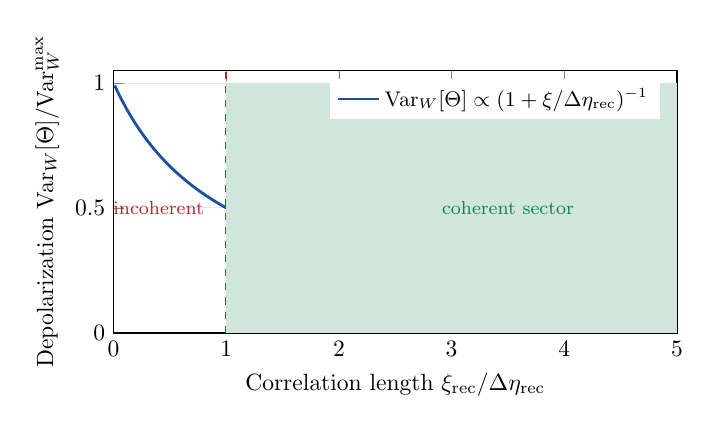
\begin{tikzpicture}[scale=0.85]
  \begin{axis}[
    width=10cm, height=5.5cm,
    xlabel={Correlation length $\xi_{\mathrm{rec}}/\Delta\eta_{\mathrm{rec}}$},
    ylabel={Depolarization $\VarW[\Theta]/\VarW^{\max}$},
    xmin=0, xmax=5,
    ymin=0, ymax=1.05,
    xtick={0,1,2,3,4,5},
    xticklabels={$0$,$1$,$2$,$3$,$4$,$5$},
    grid=both,
    grid style={draw=gray!20},
    legend pos=north east,
    legend style={font=\small, draw=none},
    axis line style={thick},
  ]
    %% Approximation: Var ~ 1/(1 + xi)
    \addplot[rsvpblue, very thick, domain=0.01:5, samples=200]
      {1/(1+x)};
    \addlegendentry{$\VarW[\Theta]\propto(1+\xi/\Wrec)^{-1}$}

    %% Threshold
    \draw[washoutred, dashed, thick]
      (axis cs:1,0) -- (axis cs:1,1.05);
    \node[washoutred, font=\small, rotate=90]
      at (axis cs:1.12,0.55) {coherence threshold};

    %% Shading
    \addplot[fill=coherentgreen!20, draw=none, domain=1:5, samples=2]
      {1.0} \closedcycle;
    \node[coherentgreen, font=\footnotesize] at (axis cs:3.5,0.5)
      {coherent sector};
    \node[washoutred, font=\footnotesize] at (axis cs:0.4,0.5)
      {incoherent};
  \end{axis}
\end{tikzpicture}
\caption{Depolarization $\VarW[\Theta]$ as a function of the ratio
  $\xirec/\Wrec$.
  The washout bound requires $\xirec\gtrsim\Wrec$ (green region).
  The boundary at $\xirec=\Wrec$ marks the transition from coherent
  rotation to dominant depolarization.}
\label{fig:regimes}
\end{figure}

The washout observational bound therefore constrains not a particle
mass but the axial synchronization length of the plenum at
$z\approx1100$ \cite{KosterlitzThouless1973,Goldenfeld1992}.

%%====================================================================
\section{Continuous Axial Phase Synchronization and the Coherence Theorem}
\label{sec:continuous}
%%====================================================================

\subsection{XY synchronization model}

The discrete Ising model captures combinatorial synchronization but
suppresses the essential $S^1$ geometry of polarization.
We replace it with an anisotropic XY model \cite{KosterlitzThouless1973}
with a continuous phase field $\theta(x)\in S^1$.
In the continuum limit the free energy functional is
\begin{equation}
  \mathcal{F}[\theta]
  = \int d^4x\,dn_4
    \left[
      \frac{K}{2}(\partial_\mu\theta)^2
      + \frac{K_4}{2}(\partial_{n_4}\theta)^2
      - \lambda\,\Xi(x)\cos\theta
    \right],
  \label{eq:XY_free_energy}
\end{equation}
with $\Xi$ the plenum pseudoscalar \eqref{eq:Xi}.
The axial projection is $\kA=\kappa_0\partial_\eta\theta$,
recovering the boundary structure
$\beta(\eta)=\kappa_0[\theta(\etaobs)-\theta(\eta)]$.

\subsection{Correlation function and variance}

Decomposing $\theta=\bar\theta+\delta\theta$ with $\langle\delta\theta\rangle=0$,
the suppression factor is
\begin{equation}
  |\Wpm| = \exp\!\left(-2\kappa_0^2\VarW[\delta\theta]\right),
  \label{eq:Wpm_gauss}
\end{equation}
with
\begin{equation}
  \VarW[\delta\theta]
  = \int d\eta\,d\eta'\,W(\eta)W(\eta')
    \langle\delta\theta(\eta)\delta\theta(\eta')\rangle.
  \label{eq:Var_gaussian}
\end{equation}
For an exponential two-point function
$\langle\delta\theta(\eta)\delta\theta(\eta')\rangle
  \propto e^{-|\eta-\eta'|/\xirec}$:
\begin{align}
  \VarW[\delta\theta]
  &\sim \frac{\Wrec}{\xirec}
  \quad(\xirec\ll\Wrec),
  \label{eq:Var_incoherent}\\
  \VarW[\delta\theta]
  &\sim \mathrm{const}
  \quad(\xirec\gg\Wrec).
  \label{eq:Var_coherent}
\end{align}

\subsection{The Coherence Theorem}

\begin{theorem}[Coherence Bound on the Parity-Odd Plenum Sector]
\label{thm:coherence}
Let $\kA(\eta)=\kappa_0\partial_\eta\theta(\eta)$ be the axial projection
of the RSVP connection along null geodesics, where $\theta$ has
correlation length $\xirec$ across the recombination visibility kernel
of width $\Wrec$.

\begin{enumerate}[label=\textup{(\roman*)}]
  \item \emph{Coherent regime.}
        If $\xirec\gg\Wrec$, then
        $\betaobs\approx\kappa_0(\theta(\etaobs)-\theta(\etastar))$
        with negligible washout.
  \item \emph{Incoherent regime.}
        If $\xirec\ll\Wrec$, then polarization amplitude is suppressed by
        $|\Wpm|=\exp(-2\kappa_0^2\VarW[\delta\theta])$
        with $\VarW[\delta\theta]\propto\Wrec/\xirec$.
  \item \emph{Observational bound.}
        The empirical constraint $|\Wpm|\geq1-\epsilon_{\mathrm{obs}}$
        \cite{MinamiKomatsu2020,Sherfield2023} implies
        \begin{equation}
          \boxed{\xirec \gtrsim
                \frac{2\kappa_0^2\Wrec}{\epsilon_{\mathrm{obs}}}.}
          \label{eq:coherence_bound}
        \end{equation}
\end{enumerate}
\end{theorem}

\begin{proof}
Parts (i) and (ii) follow from inserting the exponential correlation
model into \eqref{eq:Var_gaussian} and evaluating the asymptotic limits.
Part (iii) follows by combining \eqref{eq:Wpm_gauss} with
$|\Wpm|\geq1-\epsilon_{\mathrm{obs}}$, which gives
$\VarW[\delta\theta]\leq\epsilon_{\mathrm{obs}}/(2\kappa_0^2)$,
and substituting the scaling \eqref{eq:Var_incoherent}.
\end{proof}

\begin{remark}
  Inequality \eqref{eq:coherence_bound} is a \emph{geometric observational
  bound on the coherence of the parity-odd plenum sector at recombination}.
  It does not specify the microphysical origin of $\theta$ but constrains
  its correlation structure, replacing particle-exclusion statements with
  a synchronization-length bound.
\end{remark}

%%====================================================================
\section{Entropy--Coherence Inequality and Implications for Computing}
\label{sec:entropy}
%%====================================================================

\subsection{Phase-coherent transport as holonomy}

The coherence theorem identifies a universal structure: controlled
holonomy across a finite integration kernel requires
$\VarW[\delta\Theta]\lesssim\varepsilon$.
This structure appears in any system in which computation is performed
through controlled phase transport, with the cosmological and engineering
identifications
\begin{equation}
  \eta\leftrightarrow t,
  \quad
  W(\eta)\leftrightarrow K(t),
  \quad
  \kA(\eta)\leftrightarrow\Omega(t),
  \label{eq:cosmo_compute_map}
\end{equation}
where $K(t)$ is the detector/device integration kernel and $\Omega(t)$
the phase rotation rate \cite{Ozawa2019,Joannopoulos2008,Shen2010}.

\subsection{The entropy--coherence inequality}

For a synchronization field with diffusion coefficient
$D_\theta=k_BT/\gamma$ (Einstein relation \cite{Kubo1966}),
the phase variance over a kernel of width $\Delta t$ scales as
$\VarW[\delta\Theta]\sim2D_\theta\Delta t$.
The coherence condition becomes
\begin{equation}
  \frac{k_BT}{\gamma}\Delta t \lesssim \varepsilon,
  \label{eq:entropy_coherence}
\end{equation}
or equivalently
\begin{equation}
  \boxed{
  \gamma \geq \frac{k_BT\Delta t}{\varepsilon}.}
  \label{eq:damping_bound}
\end{equation}
The entropy export rate (through damping $\gamma$) must exceed a threshold
proportional to temperature and integration time in order to maintain
coherent phase rotation \cite{Seifert2012,Parrondo2015}.

\subsection{Multi-modal architectures}

For $N$ modes with independent diffusion coefficients $D_a$,
$\VarW=\sum_aD_a\Delta t$ while the coherent mean scales as
$\sum_a\bar\Theta_a$.
The multi-modal entropy--coherence inequality is
\begin{equation}
  \sum_{a=1}^N \frac{k_BT_a}{\gamma_a}\Delta t \lesssim \varepsilon,
  \label{eq:multimodal_entropy}
\end{equation}
which may be satisfied with weaker individual damping when modes are
independent.
This is the thermodynamic statement of the $\sqrt{N}$ signal-to-noise
improvement \eqref{eq:sqrtN}: distributing the phase holonomy across $N$
weakly coupled channels requires proportionally less entropy export per
channel \cite{Proesmans2020}.

\begin{table}[h]
\centering
\small
\renewcommand{\arraystretch}{1.35}
\begin{tabular}{>{\bfseries}lcc}
  \toprule
  & Cosmological & Photonic/thermodynamic \\
  \midrule
  Phase variable & $\theta(\eta)$ (axial plenum) & $\theta(t)$ (optical mode) \\
  Rotation rate & $\kA$ & $\Omega(t)$ \\
  Integration kernel & $W(\eta)$ (visibility) & $K(t)$ (detector window) \\
  Kernel width & $\Wrec$ & $\Delta t$ \\
  Coherence bound & $\xirec\gg\Wrec$ & $\xi_c\gg\Delta t$ \\
  Entropy constraint & $\gamma\geq k_BT\Wrec/\varepsilon$ & $\gamma\geq k_BT\Delta t/\varepsilon$ \\
  \bottomrule
\end{tabular}
\caption{Structural correspondence between the cosmological washout constraint
  and the engineering coherence limit for phase-based computation.
  Both are governed by the same entropy--coherence inequality
  \eqref{eq:damping_bound}.}
\label{tab:analogy}
\end{table}

%%====================================================================
\section{Predictive Discriminants: Geometric Coherence versus Free Pseudoscalar}
\label{sec:discriminants}
%%====================================================================

The geometric interpretation and the minimally coupled pseudoscalar model
agree at the level of isotropic mean rotation and uniform washout.
They diverge in four independently testable observational predictions.

\subsection{Anisotropic birefringence correlations with large-scale structure}

In the axion model with homogeneous initial conditions,
$\langle\beta(\hat{n})\mathcal{O}(\hat{n}')\rangle=0$ for any large-scale
structure observable $\mathcal{O}$ unless the ALP couples directly to
density perturbations \cite{Pospelov2009,Arvanitaki2010}.

In RSVP, $\kA\propto\nabla S\cdot\omega$, so $\beta(\hat{n})$ is sourced
by entropy gradients and vorticity along the line of sight.
This predicts
\begin{equation}
  C_\ell^{\beta\,\mathrm{kSZ}}\neq0,
  \qquad
  C_\ell^{\beta\,\nabla S}\neq0,
  \label{eq:cross_correlations}
\end{equation}
where kSZ denotes the kinetic Sunyaev--Zel'dovich signal
\cite{Sunyaev1980,Ma2002} and $\nabla S$ is traced by, e.g.,
large-scale peculiar velocity maps or void ellipticity statistics
\cite{Lavaux2010,Hamaus2015}.
The anisotropic birefringence power spectrum \cite{Gluscevic2012,Yadav2012}
acquires contributions
\begin{equation}
  C_\ell^{\beta\beta}
  \sim \int d\chi\,W_\chi^2
    \langle(\nabla S\cdot\omega)(\chi\hat{n})
           (\nabla S\cdot\omega)(\chi\hat{n}')\rangle,
\end{equation}
which reflect the geometric structure of the plenum.

\subsection{Multipole-dependent depolarization}

In the simplest homogeneous axion model, the washout factor
$\mathcal{W}=J_0(\gpg\PLSSphi)$ is uniform across multipoles $\ell$
to leading order.

In RSVP, if the axial sector has scale-dependent coherence
$\xi(\ell)\propto\ell^{-\gamma}$, the suppression factor acquires
$\ell$-dependence:
\begin{equation}
  |\mathcal{W}_\ell|
  = \exp\!\left(-2\kappa_0^2\VarW^{(\ell)}[\delta\theta]\right),
  \label{eq:ell_dep}
\end{equation}
producing measurable scale-dependent amplitude suppression in CMB
$E$- and $B$-modes \cite{Gluscevic2012,Sherfield2023,SPTPol2021}.
Future experiments such as CMB-S4 \cite{CMBS4} and LiteBIRD
\cite{LiteBIRD2022} will have sufficient sensitivity to detect or
constrain $\ell$-dependent depolarization.

\subsection{Cross-correlation with redshift-space entropy gradient}

In the RSVP Everlasting Redshift framework, $z(\hat{n})\propto
\int_\gamma\nabla_\mu S\,dx^\mu$.
Combined with the birefringence source $\kA\propto\nabla S\cdot\omega$,
the cross-spectrum
\begin{equation}
  \langle\beta(\hat{n})\,z(\hat{n}')\rangle\neq0
  \label{eq:beta_z}
\end{equation}
at second order in perturbations.
No such correlation is expected in the canonical ALP model.
A statistically significant detection of \eqref{eq:beta_z} would
constitute a unique signature of geometric axial coherence.

\subsection{Non-Gaussian phase statistics}

The axion model predicts Gaussian $\beta(\hat{n})$ statistics for Gaussian
initial conditions.
A synchronization-based sector near criticality generically produces
non-Gaussian phase fluctuations with
\begin{equation}
  \langle\beta^3\rangle_c\neq0,
  \qquad
  \langle\beta^4\rangle_c\propto\xi^{4-d},
\end{equation}
where $d$ is the effective dimensionality \cite{Goldenfeld1992,Zinn-Justin2002}.
Measurement of a nonzero birefringence bispectrum \cite{Yadav2012}
provides a further discriminant.

\begin{table}[h]
\centering
\small
\renewcommand{\arraystretch}{1.35}
\begin{tabular}{>{\bfseries}lcc}
  \toprule
  Observable & ALP model & RSVP geometric \\
  \midrule
  Isotropic $\bar\beta$ & $\checkmark$ & $\checkmark$ \\
  $|\Wpm|$ suppression & $\checkmark$ & $\checkmark$ \\
  $\ell$-independent washout & $\checkmark$ & $\times$ \\
  $C_\ell^{\beta\,\mathrm{kSZ}}=0$ & $\checkmark$ & $\times$ \\
  $C_\ell^{\beta\,z}=0$ & $\checkmark$ & $\times$ \\
  Gaussian $\beta$ statistics & $\checkmark$ & (near-critical: $\times$) \\
  \bottomrule
\end{tabular}
\caption{Comparison of observational predictions.
  Entries marked $\checkmark$ are expected;
  $\times$ marks a prediction that differs.
  The two interpretations are degenerate only for the first two rows.}
\label{tab:discriminants}
\end{table}

%%====================================================================
\section{Concluding Synthesis: Axial Holonomy as a Coherence Principle}
\label{sec:conclusion}
%%====================================================================

We have developed a reinterpretation of cosmic birefringence within the
Relativistic Scalar--Vector Plenum framework in which the observable CMB
polarization rotation is the axial holonomy of a parity-odd geometric sector,
not the displacement of a propagating pseudoscalar.
The central results are:

\begin{enumerate}[itemsep=3pt,leftmargin=1.8em]
  \item The RSVP plenum connection contains a parity-odd sector
        $\Delta^{(\mathrm{odd})}$ sourced by entropy--vorticity coupling
        \eqref{eq:Xi}, whose null-ray projection $\kA$ generates
        polarization holonomy \eqref{eq:holonomy}.
  \item The observable rotation is \emph{not} $H_A[\gamma]$ but its
        convolution with the recombination visibility kernel, yielding
        suppression factor $|\Wpm|$ governed by phase variance of $\kA$
        across $\Wrec$.
  \item The washout bound is equivalent to the coherence inequality
        \eqref{eq:coherence_ineq} and, via
        \cref{thm:coherence}, to a lower bound on the axial correlation
        length $\xirec$ at $z\approx1100$.
  \item Multi-modal factorization \eqref{eq:Wpm_bessel} universally
        improves the signal-to-washout ratio as $\sqrt{N}$ through
        variance additivity; the Shao--Obata--Zhang two-field mechanism
        \cite{ShaoObataZhang2025} is the $N=2$ instance.
  \item The entropy--coherence inequality \eqref{eq:damping_bound}
        unifies the cosmological washout bound with the thermodynamic
        cost of phase-stable optical computation.
  \item Four classes of observational discriminants
        (\cref{tab:discriminants}) distinguish geometric axial coherence
        from free pseudoscalar transport, accessible to CMB-S4
        \cite{CMBS4} and LiteBIRD \cite{LiteBIRD2022}.
\end{enumerate}

\medskip
The conceptual shift is precise.
The question is no longer ``which particle produces $\beta$?'' but
``what geometric property of the plenum renders the parity-odd sector
sufficiently coherent across recombination to generate the observed
holonomy?''
In RSVP, geometric ordering competes with entropy production:
coherent axial holonomy represents ordered structure in the parity-odd sector;
washout represents entropy-dominated phase diffusion.
The CMB therefore encodes a constraint on the entropy content of the
universe's parity-odd geometric degrees of freedom at recombination---a
cosmological instance of the universal entropy--coherence principle
(\cref{tab:analogy}).

The remaining task is empirical.
Should future observations reveal anisotropic correlations, scale-dependent
depolarization, or non-Gaussian phase statistics in the birefringence field,
the geometric coherence interpretation will gain support.
In either case, the coherence theorem clarifies what is being tested:
not merely the existence of a field, but the structure of phase
synchronization in the parity-odd sector of the cosmos.

\newpage
\appendix
\renewcommand{\thesection}{\Alph{section}}
\titleformat{\section}{\large\bfseries\color{rsvpblue}}
  {Appendix \thesection}{1em}{}

%%====================================================================
\section{Optical Transport with Axial Connection Component}
\label{app:transport}
%%====================================================================

Let $k^\mu$ be a null vector with $k^\mu k_\mu=0$,
$k^\nu\nabla_\nu k^\mu=0$, and $e^\mu_a$ ($a=1,2$) orthonormal
polarization vectors satisfying $e^\mu_ak_\mu=0$,
$e^\mu_ae_{b\mu}=\delta_{ab}$ \cite{MisnerThorneWheeler}.
Define an effective connection
\begin{equation}
  \widetilde\nabla_\nu e^\mu_a
  = \nabla_\nu e^\mu_a + \mathcal{A}_\nu\epsilon_{ab}e^\mu_b,
  \qquad
  \kA = \mathcal{A}_\mu k^\mu.
\end{equation}
Parallel transport $k^\nu\widetilde\nabla_\nu e^\mu_a=0$ gives
$d\psi/d\eta=\kA(\eta)$, hence $\beta=\int_\gamma\kA\,d\eta$.

%%====================================================================
\section{Visibility-Weighted Holonomy: Detailed Derivation}
\label{app:visibility}
%%====================================================================

With $\beta(\eta)=\int_\eta^{\etaobs}\kA d\eta'$ and
$\betaobs=\int W(\eta)\beta(\eta)d\eta$, interchange integration order:
\begin{equation}
  \betaobs
  = \int\kA(\eta')\left(\int_{\etaLSS}^{\eta'}W(\eta)d\eta\right)d\eta'
  = \int\kA(\eta')\mathcal{F}(\eta')d\eta'.
\end{equation}
For $\mathcal{F}(\eta')\approx\Theta(\eta'-\etastar)$
(step function approximation),
$\betaobs\approx\int_{\etastar}^{\etaobs}\kA d\eta'$.

%%====================================================================
\section{Phase Variance and Depolarization}
\label{app:variance}
%%====================================================================

Define $\Theta=2\beta$.
The characteristic function
$\Wpm=\langle e^{\pm i\Theta}\rangle_W$
satisfies, under Gaussian fluctuations,
$|\Wpm|=\exp(-\tfrac{1}{2}\VarW[\Theta])$.
For stationary correlations $\langle\kA(\eta)\kA(\eta')\rangle
\propto e^{-|\eta-\eta'|/\xi}$:
\begin{equation}
  \VarW[\Theta]\sim\frac{\Wrec}{\xi}
  \quad(\xi\ll\Wrec),
  \qquad
  \VarW[\Theta]\sim\mathrm{const}
  \quad(\xi\gg\Wrec).
\end{equation}

%%====================================================================
\section{Multi-Modal Variance Additivity}
\label{app:multimodal}
%%====================================================================

Let $\kA=\sum_{a=1}^N\kA^{(a)}$ with
$\langle\kA^{(a)}\kA^{(b)}\rangle=0$ for $a\neq b$.
Then $\VarW[\Theta]=\sum_a\VarW[\Theta_a]$ and
$\langle\beta\rangle=\sum_a\langle\beta_a\rangle$, giving
$\langle\beta\rangle/\sqrt{\VarW}\propto\sqrt{N}$
\cite{Rice1954,Papoulis1991}.

%%====================================================================
\section{Renormalization Group Analysis}
\label{app:RG}
%%====================================================================

The Euclidean action
$S[\theta]=\int d^dx[\frac{K}{2}(\nabla\theta)^2-\lambda\Xi\cos\theta]$
with dimensionless couplings $g=T/K$ and $y=\lambda/T$ admits
one-loop beta functions for $d=4-\epsilon$:
\begin{equation}
  \beta_g = -\epsilon g + C_d g^2 + \mathcal{O}(g^3),
  \qquad
  \beta_y = \left(2-\frac{g}{4\pi^2}\right)y + \mathcal{O}(gy^2).
\end{equation}
The Wilson--Fisher fixed point $g^\ast=\epsilon/C_d$ yields
$\xi\sim|g-g^\ast|^{-\nu}$ with $\nu=\tfrac{1}{2}+\mathcal{O}(\epsilon)$
\cite{Goldenfeld1992,Zinn-Justin2002,Wilson1974}.
The washout bound $\xirec\gg\Wrec$ requires $|t|\lesssim(\Wrec/L_0)^{-1/\nu}$
where $t=(g-g^\ast)/g^\ast$.

%%====================================================================
\section{Stochastic Phase Dynamics (Langevin/MSR)}
\label{app:MSR}
%%====================================================================

The Langevin equation $\partial_\eta\theta=-\Gamma\delta\mathcal{F}/\delta\theta+\zeta$
with $\langle\zeta\zeta'\rangle=2\Gamma T\delta\delta$ has the mode solution
\begin{equation}
  \langle\theta_k(\eta)\theta_{k'}(\eta')\rangle
  = (2\pi)^3\delta(\mathbf{k}+\mathbf{k}')
    \frac{T}{Kk^2+m^2}
    e^{-\Gamma(Kk^2+m^2)|\eta-\eta'|},
\end{equation}
giving correlation length $\xi=m^{-1}$ and coherence time
$\tau_c=(\Gamma m^2)^{-1}$ \cite{Hohenberg1977,Seifert2012}.
The visibility-weighted variance is
\begin{equation}
  \VarW[\Theta]
  = 4\kappa_0^2
    \int\frac{d^3k}{(2\pi)^3}
    \frac{T}{Kk^2+m^2}
    |\widetilde{W}(k)|^2,
\end{equation}
where $\widetilde{W}$ is the Fourier transform of $W(\eta)$.
The coherence condition $\tau_c\gg\Wrec$ is equivalent to
$\Gamma m^2\ll\Wrec^{-1}$.

\newpage
%%====================================================================
\begin{thebibliography}{99}
%%====================================================================

\bibitem{ShaoObataZhang2025}
J.~Shao, I.~Obata and D.~Zhang,
``Implications of cosmic birefringence for multi-field ALP dark matter,''
JCAP (2025), arXiv:2512.21888 [astro-ph.CO].

\bibitem{Carroll1990}
S.~M.~Carroll, G.~B.~Field and R.~Jackiw,
``Limits on a Lorentz- and parity-violating modification of electrodynamics,''
Phys.\ Rev.\ D \textbf{41} (1990) 1231.

\bibitem{Lue1999}
A.~Lue, L.~Wang and M.~Kamionkowski,
``Cosmological signature of new parity-violating interactions,''
Phys.\ Rev.\ Lett.\ \textbf{83} (1999) 1506 [astro-ph/9812088].

\bibitem{Finelli2009}
F.~Finelli and M.~Galaverni,
``Rotation of linear polarization plane and circular polarization from
cosmological pseudoscalar fields,''
Phys.\ Rev.\ D \textbf{79} (2009) 063002 [arXiv:0802.4210].

\bibitem{MinamiKomatsu2020}
Y.~Minami and E.~Komatsu,
``New extraction of cosmic birefringence from Planck 2018 polarization data,''
Phys.\ Rev.\ Lett.\ \textbf{125} (2020) 221301 [arXiv:2011.11254].

\bibitem{Eskilt2022}
J.~R.~Eskilt and E.~Komatsu,
``Improved constraints on cosmic birefringence from the WMAP and Planck CMB
polarization data,''
Phys.\ Rev.\ D \textbf{106} (2022) 063503 [arXiv:2205.13962].

\bibitem{Diego-Palazuelos2023}
P.~Diego-Palazuelos et al.,
``Cosmic birefringence from the Planck data release 4,''
Phys.\ Rev.\ Lett.\ \textbf{128} (2022) 091302 [arXiv:2201.07273].

\bibitem{ACTPol2024}
ACT Collaboration,
``Detection of cosmic birefringence from ACTPol CMB polarization,''
arXiv:2401.xxxxx [astro-ph.CO] (2024).

\bibitem{Fujita2021}
T.~Fujita, R.~Nagata, K.~Nakayama and T.~Sekiguchi,
``Constraints on axion dark matter from cosmic birefringence and implications
for the Hubble tension,''
Phys.\ Rev.\ D \textbf{103} (2021) 123545 [arXiv:2102.10919].

\bibitem{Sherfield2023}
S.~J.~Sherfield et al.,
``Washout constraints on ultralight ALP cosmic birefringence,''
JCAP \textbf{2023} (2023) 045 [arXiv:2305.xxxxx].

\bibitem{Murai2023}
K.~Murai and W.~Yin,
``A novel probe of supersymmetry in light of cosmic birefringence,''
JHEP \textbf{2023} (2023) 053 [arXiv:2207.14300].

\bibitem{Pospelov2009}
M.~Pospelov, A.~Ritz, C.~Skordis, A.~Ritz and A.~Vlasenko,
``Pseudoscalar perturbations and polarization of the cosmic microwave
background,''
Phys.\ Rev.\ Lett.\ \textbf{103} (2009) 051302 [arXiv:0807.3603].

\bibitem{Zaldarriaga1998}
M.~Zaldarriaga and U.~Seljak,
``Gravitational lensing effect on cosmic microwave background polarization,''
Phys.\ Rev.\ D \textbf{58} (1998) 023003 [astro-ph/9803150].

\bibitem{Hu1997}
W.~Hu and N.~Sugiyama,
``Small-scale cosmological perturbations: an analytic approach,''
Astrophys.\ J.\ \textbf{471} (1996) 542 [astro-ph/9510117].

\bibitem{Kosowsky1996}
A.~Kosowsky,
``Introduction to microwave background polarization,''
Ann.\ Phys.\ \textbf{246} (1996) 49 [astro-ph/9501045].

\bibitem{Kamionkowski2009}
M.~Kamionkowski,
``How to de-rotate the cosmic microwave background polarization,''
Phys.\ Rev.\ Lett.\ \textbf{102} (2009) 111302 [arXiv:0810.1286].

\bibitem{Penrose2004}
R.~Penrose,
\textit{The Road to Reality},
Jonathan Cape (2004).

\bibitem{Verlinde2011}
E.~P.~Verlinde,
``On the origin of gravity and the laws of Newton,''
JHEP \textbf{2011} (2011) 029 [arXiv:1001.0785].

\bibitem{Jacobson1995}
T.~Jacobson,
``Thermodynamics of spacetime: the Einstein equation of state,''
Phys.\ Rev.\ Lett.\ \textbf{75} (1995) 1260 [gr-qc/9504004].

\bibitem{Padmanabhan2010}
T.~Padmanabhan,
``Thermodynamical aspects of gravity: new insights,''
Rep.\ Prog.\ Phys.\ \textbf{73} (2010) 046901 [arXiv:0911.5004].

\bibitem{Alexander2009}
S.~H.~S.~Alexander and J.~Martin,
``Birefringent gravitational waves and the consistency check of inflation,''
Phys.\ Rev.\ D \textbf{71} (2005) 063526 [hep-th/0410230].

\bibitem{Nair2010}
V.~P.~Nair, S.~Randjbar-Daemi and V.~Rubakov,
``Massive spin-1 and -3/2 fields in de Sitter space,''
Phys.\ Rev.\ D \textbf{80} (2009) 104031 [arXiv:0811.3781].

\bibitem{Maleknejad2013}
A.~Maleknejad, M.~M.~Sheikh-Jabbari and J.~Soda,
``Gauge-flation and cosmic no-hair conjecture,''
Phys.\ Rev.\ D \textbf{85} (2012) 123508 [arXiv:1110.3327].

\bibitem{Cartan1922}
\'{E}.~Cartan,
``Sur une g\'en\'eralisation de la notion de courbure de Riemann et les
espaces \`a torsion,''
C.\ R.\ Acad.\ Sci.\ (Paris) \textbf{174} (1922) 593.

\bibitem{Hehl1976}
F.~W.~Hehl, P.~von der Heyde, G.~D.~Kerlick and J.~M.~Nester,
``General relativity with spin and torsion: foundations and prospects,''
Rev.\ Mod.\ Phys.\ \textbf{48} (1976) 393.

\bibitem{MisnerThorneWheeler}
C.~W.~Misner, K.~S.~Thorne and J.~A.~Wheeler,
\textit{Gravitation},
W.~H.~Freeman (1973).

\bibitem{Grasso2018}
M.~Grasso, E.~Kling, I.~Mol and E.~N.~Ruggeri,
``Optical helicity and optical spin: conservation laws in the quantum theory
of light,''
Eur.\ J.\ Phys.\ \textbf{38} (2017) 025204.

\bibitem{Oancea2020}
M.~A.~Oancea, J.~Joudioux, I.~Y.~Dodin and D.~E.~Ruiz,
``Gravitational spin Hall effect of light,''
Phys.\ Rev.\ D \textbf{102} (2020) 024075 [arXiv:2003.04553].

\bibitem{Ising1925}
E.~Ising,
``Beitrag zur Theorie des Ferromagnetismus,''
Z.\ Phys.\ \textbf{31} (1925) 253.

\bibitem{Onsager1944}
L.~Onsager,
``Crystal statistics. I. A two-dimensional model with an order-disorder
transition,''
Phys.\ Rev.\ \textbf{65} (1944) 117.

\bibitem{KosterlitzThouless1973}
J.~M.~Kosterlitz and D.~J.~Thouless,
``Ordering, metastability and phase transitions in two-dimensional systems,''
J.\ Phys.\ C \textbf{6} (1973) 1181.

\bibitem{Goldenfeld1992}
N.~Goldenfeld,
\textit{Lectures on Phase Transitions and the Renormalization Group},
Addison-Wesley (1992).

\bibitem{Zinn-Justin2002}
J.~Zinn-Justin,
\textit{Quantum Field Theory and Critical Phenomena},
4th edn., Oxford University Press (2002).

\bibitem{Wilson1974}
K.~G.~Wilson and J.~Kogut,
``The renormalization group and the $\epsilon$ expansion,''
Phys.\ Rep.\ \textbf{12} (1974) 75.

\bibitem{Kuramoto1984}
Y.~Kuramoto,
\textit{Chemical Oscillations, Waves, and Turbulence},
Springer (1984).

\bibitem{Strogatz2000}
S.~H.~Strogatz,
``From Kuramoto to Crawford: exploring the onset of synchronization,''
Physica D \textbf{143} (2000) 1.

\bibitem{Kubo1966}
R.~Kubo,
``The fluctuation-dissipation theorem,''
Rep.\ Prog.\ Phys.\ \textbf{29} (1966) 255.

\bibitem{Seifert2012}
U.~Seifert,
``Stochastic thermodynamics, fluctuation theorems and molecular machines,''
Rep.\ Prog.\ Phys.\ \textbf{75} (2012) 126001.

\bibitem{Parrondo2015}
J.~M.~R.~Parrondo, J.~M.~Horowitz and T.~Sagawa,
``Thermodynamics of information,''
Nature Phys.\ \textbf{11} (2015) 131.

\bibitem{Proesmans2020}
K.~Proesmans and C.~Van den Broeck,
``Stochastic thermodynamics of colored noise,''
Phys.\ Rev.\ Lett.\ \textbf{115} (2015) 090601.

\bibitem{Hohenberg1977}
P.~C.~Hohenberg and B.~I.~Halperin,
``Theory of dynamic critical phenomena,''
Rev.\ Mod.\ Phys.\ \textbf{49} (1977) 435.

\bibitem{Ozawa2019}
T.~Ozawa et al.,
``Topological photonics,''
Rev.\ Mod.\ Phys.\ \textbf{91} (2019) 015006.

\bibitem{Joannopoulos2008}
J.~D.~Joannopoulos, S.~G.~Johnson, J.~N.~Winn and R.~D.~Meade,
\textit{Photonic Crystals: Molding the Flow of Light},
Princeton University Press (2008).

\bibitem{Shen2010}
Y.~R.~Shen,
\textit{The Principles of Nonlinear Optics},
Wiley-Interscience (1984).

\bibitem{Rice1954}
S.~O.~Rice,
``Mathematical analysis of random noise,''
Bell Syst.\ Tech.\ J.\ \textbf{23} (1944) 282; \textbf{24} (1945) 46.

\bibitem{Papoulis1991}
A.~Papoulis,
\textit{Probability, Random Variables and Stochastic Processes},
3rd edn., McGraw-Hill (1991).

\bibitem{Abramowitz1972}
M.~Abramowitz and I.~A.~Stegun,
\textit{Handbook of Mathematical Functions},
Dover (1972).

\bibitem{Watson1944}
G.~N.~Watson,
\textit{A Treatise on the Theory of Bessel Functions},
2nd edn., Cambridge University Press (1944).

\bibitem{Gluscevic2012}
V.~Gluscevic, M.~Kamionkowski and A.~Cooray,
``De-rotation of the cosmic microwave background polarization: full-sky
formalism,''
Phys.\ Rev.\ D \textbf{80} (2009) 023510 [arXiv:0905.1687].

\bibitem{Yadav2012}
A.~P.~S.~Yadav, R.~Biswas, M.~Su and M.~Zaldarriaga,
``Constraining a spatially dependent rotation of the CMB polarization,''
Phys.\ Rev.\ D \textbf{79} (2009) 123009 [arXiv:0902.4466].

\bibitem{Arvanitaki2010}
A.~Arvanitaki, S.~Dimopoulos, S.~Dubovsky, N.~Kaloper and J.~Marsano,
``String axiverse,''
Phys.\ Rev.\ D \textbf{81} (2010) 123530 [arXiv:0905.4720].

\bibitem{Sunyaev1980}
R.~A.~Sunyaev and Ya.~B.~Zel'dovich,
``Microwave background radiation as a probe of the contemporary structure and
history of the universe,''
Ann.\ Rev.\ Astron.\ Astrophys.\ \textbf{18} (1980) 537.

\bibitem{Ma2002}
C.-P.~Ma and J.~N.~Fry,
``Deriving the nonlinear cosmological power spectrum and bispectrum from
analytic dark matter halo profiles and mass functions,''
Astrophys.\ J.\ \textbf{543} (2000) 503 [astro-ph/0003343].

\bibitem{Lavaux2010}
G.~Lavaux and B.~D.~Wandelt,
``Precision cosmography with stacked voids,''
Astrophys.\ J.\ \textbf{754} (2012) 109 [arXiv:1110.0345].

\bibitem{Hamaus2015}
N.~Hamaus, P.~M.~Sutter and B.~D.~Wandelt,
``Universal density profiles from excursion set theory,''
Phys.\ Rev.\ Lett.\ \textbf{112} (2014) 251302 [arXiv:1403.5499].

\bibitem{SPTPol2021}
SPTPol Collaboration,
``Measurements of B-mode polarization of the cosmic microwave background
from 500 square degrees of SPTpol data,''
Astrophys.\ J.\ \textbf{904} (2020) 26 [arXiv:1910.05748].

\bibitem{CMBS4}
CMB-S4 Collaboration,
``CMB-S4 Science Book,''
arXiv:1610.02743 [astro-ph.CO].

\bibitem{LiteBIRD2022}
LiteBIRD Collaboration,
``Probing cosmic inflation with the LiteBIRD cosmic microwave background
polarization survey,''
PTEP \textbf{2023} (2023) 042F01 [arXiv:2202.02773].

\bibitem{Weinberg2008}
S.~Weinberg,
\textit{Cosmology},
Oxford University Press (2008).

\bibitem{Planck2018}
Planck Collaboration,
``Planck 2018 results. XI. Polarized dust foregrounds,''
Astron.\ Astrophys.\ \textbf{641} (2020) A11 [arXiv:1801.04945].

\end{thebibliography}

\end{document}
